\documentclass[12pt,english]{article}
\usepackage[T1]{fontenc}
\usepackage{babel}
\usepackage[margin=0.8 in]{geometry}
\usepackage{caption}
\usepackage{subfig}
\usepackage{longtable}
\usepackage{natbib}
\linespread{1.15}
\usepackage{tikz}
\usepackage{setspace}
\usepackage{multirow}
\usepackage{multicol}
\usepackage{csquotes}
%\usepackage{mathds}
% ------
% Fonts and typesetting settings


%\usepackage[sc]{mathpazo}
\usepackage{titling}									
\usepackage{float}
\usepackage{pdflscape}
\usepackage[toc]{appendix}
\renewcommand{\appendixtocname}{Appendices}
%\renewcommand{\appendixsection}{\normalfont\bfseries}
\usepackage{amsmath, amsthm, amsfonts}


\newcommand{\subtitle}[1]{%
  \posttitle{%
    \par\end{center}
    \begin{center}\large#1\end{center}
    \vskip0.5em}%
}

\usepackage{booktabs}												
\usepackage{natbib}                                                 
\usepackage{graphics,epsfig}						
% -----
% ------

% Node styles
\tikzset{
% Two node styles for game trees: solid and hollow
solid node/.style={circle,draw,inner sep=1.5,fill=black},
hollow node/.style={circle,draw,inner sep=1.5}
}


% Maketitle metadata
\author{
Natalia Serna
   }
 \title{Problem set 5}

\date{}
%%%%%%%%%%%%%%%%%%%%%%%%
\begin{document}

\maketitle


\begin{enumerate}
\item 
\begin{enumerate}
\item The sequential game of this interaction between incumbent and entrant is shown below:
\begin{center}
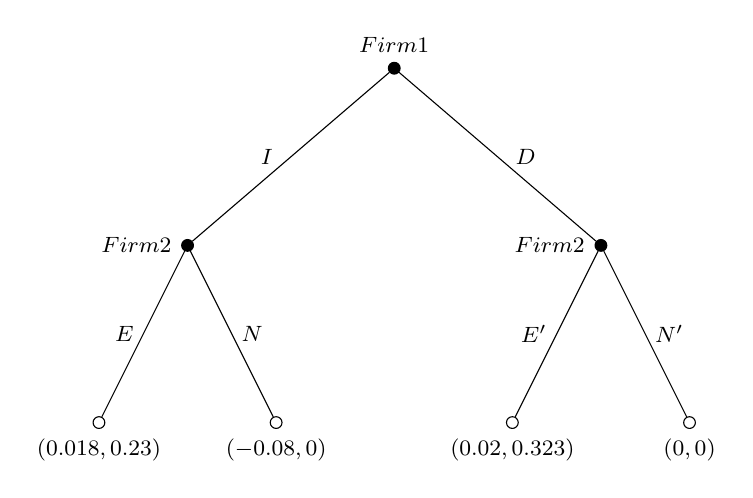
\begin{tikzpicture}[scale=1.5,font=\footnotesize]
% Specify spacing for each level of the tree
\tikzstyle{level 1}=[level distance=15mm,sibling distance=35mm]
\tikzstyle{level 2}=[level distance=15mm,sibling distance=15mm]
% The Tree
\node(0)[solid node,label=above:{$Firm 1$}]{}
child{node(1)[solid node,label=left:{$Firm 2$}]{}
child{node[hollow node,label=below:{$(0.018,0.23)$}]{} edge from parent node[left]{$E$}}
child{node[hollow node,label=below:{$(-0.08,0)$}]{} edge from parent node[right]{$N$}}
edge from parent node[left,xshift=-3]{$I$}
}
child{node(2)[solid node,label=left:{$Firm 2$}]{}
child{node[hollow node,label=below:{$(0.02,0.323)$}]{} edge from parent node[left]{$E'$}}
child{node[hollow node,label=below:{$(0,0)$}]{} edge from parent node[right]{$N'$}}
edge from parent node[right,xshift=3]{$D$}
};
% information set
%\draw[dashed,rounded corners=10];
% specify mover at 2nd information set
\end{tikzpicture}
\end{center}

To compute the payoffs of this game first we find the best response of Firm 2 $p_{2}(p_{1})$ and then plug it into the profits of Firm 1 to find its choice of price. The best response of firm 2 is:

\begin{align}
&max_{p_{2}}\ \ \pi_{2}=(1-2p_{2}+p_{1})p_{2}\nonumber\\
&\textcolor{blue}{p_{2}=\frac{1+p_{1}}{4}}\nonumber
\end{align}

Given this, firm 1's best response and payoffs to both players in each final node are:

\begin{itemize}
\item (I,E)
\begin{align}
&max_{p_{1}}\ \ \pi_{1}=\left(1-2p_{1}+\frac{1+p_{1}}{4}\right)p_{1}-0.205\nonumber\\
&\textcolor{blue}{p_{1}=\frac{5}{14}}, \ \ \textcolor{blue}{p_{2}=\frac{19}{56}}\nonumber\\
& \textcolor{blue}{\pi_{1}=0.018}, \ \ \textcolor{blue}{\pi_{2}=0.23}\nonumber
\end{align}

\item (D,E)
\begin{align}
&max_{p_{1}}\ \ \pi_{1}=\left(1-2p_{1}+\frac{1+p_{1}}{4}\right)(p_{1}-0.5)\nonumber\\
&\textcolor{blue}{p_{1}=\frac{17}{28}}, \ \ \textcolor{blue}{p_{2}=\frac{45}{112}}\nonumber\\
& \textcolor{blue}{\pi_{1}=0.0201}, \ \ \textcolor{blue}{\pi_{2}=0.323}\nonumber
\end{align}

\item (I,N)
\begin{align}
&max_{p_{1}}\ \ \pi_{1}=\left(1-2p_{1}\right)p_{1}-0.205\nonumber\\
&\textcolor{blue}{p_{1}=\frac{1}{4}}, \ \ \textcolor{blue}{p_{2}=0}\nonumber\\
& \textcolor{blue}{\pi_{1}=-0.08}, \ \ \textcolor{blue}{\pi_{2}=0}\nonumber
\end{align}

\item (D,N)
\begin{align}
&max_{p_{1}}\ \ \pi_{1}=\left(1-2p_{1}\right)(p_{1}-0.5)\nonumber\\
&\textcolor{blue}{p_{1}=\frac{1}{2}}, \ \ \textcolor{blue}{p_{2}=0}\nonumber\\
& \textcolor{blue}{\pi_{1}=0}, \ \ \textcolor{blue}{\pi_{2}=0}\nonumber
\end{align}
\end{itemize}

By backward induction, there is a unique subgame perfect equilibrium $\{D,(EE')\}$. Therefore, Firm 1 does not invest.

\item When the entrant does not observe the incumbent's investment choice, this becomes a simultaneous-move game. The solution concept is  then Nash equilibrium and not subgame perfection. To determine whether a strategy profile is an equilibrium we need to check that there are no profitable one-shot deviations. 

In this game a strategy for player 1 is 
\[
s_{1}\in\{(I, p)| I=\mathbf{1}\{Invest>0\}, p\{0,1\}\to\mathcal{R}_{+}]\}
\]

And for player 2:
\[
s_{2}\in p:\mathcal{R}_{+}\to\mathcal{R}_{+}
\]
\item  
The best response of firm 2 is:

\begin{align}
&max_{p_{2}}\ \ \pi_{2}=(1-2p_{2}+p_{1})p_{2}\nonumber\\
&\textcolor{blue}{p_{2}=\frac{1+p_{1}}{4}}\nonumber
\end{align}

Given this, firm 1's best response and payoffs to both players in each final node are:

\begin{itemize}
\item (I,E)
\begin{align}
&max_{p_{1}}\ \ \pi_{1}=\left(1-2p_{1}+p_{2}\right)p_{1}-0.205\nonumber\\
&\textcolor{blue}{p_{1}=\frac{1+p_{2}}{4}}\nonumber\\
&\textcolor{blue}{p_{1}=p_{2}=\frac{1}{3}}\nonumber\\
&\textcolor{blue}{\pi^{eq}_{1}=0.0172,\ \ \pi_{2}=2/9}\nonumber
\end{align}
Now consider a one-shot deviation for firm 1 into not investing:
\begin{align}
&max_{p_{1}}\ \ \pi_{1}=\left(1-2p_{1}+1/3\right)(p_{1}-0.5)\nonumber\\
&\textcolor{blue}{p_{1}=7/12}\nonumber\\
&\textcolor{blue}{\pi^{dev}_{1}=1/72,\ \ \pi_{2}=11/36}\nonumber
\end{align}
\textcolor{blue}{Since $\pi^{eq}_{1}>\pi^{dev}_{1}$ then firm 1 investing is an equilibrium.}


\item (D,E)
\begin{align}
&max_{p_{1}}\ \ \pi_{1}=\left(1-2p_{1}+p_{2}\right)(p_{1}-0.5)\nonumber\\
&\textcolor{blue}{p_{1}=\frac{2+p_{2}}{4}}\nonumber\\
&\textcolor{blue}{p_{1}=\frac{3}{5},\ \ p_{2}=\frac{2}{5}}\nonumber\\
&\textcolor{blue}{\pi^{eq}_{1}=1/50,\ \ \pi_{2}=8/25}\nonumber
\end{align}
Now consider a one-shot deviation from firm 1 into investing:
\begin{align}
&max_{p_{1}}\ \ \pi_{1}=\left(1-2p_{1}+2/5\right)p_{1}-0.205\nonumber\\
&\textcolor{blue}{p_{1}=7/20}\nonumber\\
&\textcolor{blue}{\pi^{dev}_{1}=0.04,\ \ \pi_{2}=0.22}\nonumber
\end{align}
\textcolor{blue}{Since $\pi^{dev}_{1}>\pi^{eq}_{1}$ then there exists a profitable deviation in which firm 1 invests.}


\item (I,N)
\begin{align}
&max_{p_{1}}\ \ \pi_{1}=\left(1-2p_{1}\right)p_{1}-0.205\nonumber\\
&\textcolor{blue}{p_{1}=\frac{1}{4}}, \ \ \textcolor{blue}{p_{2}=0}\nonumber\\
& \textcolor{blue}{\pi_{1}=-0.08}, \ \ \textcolor{blue}{\pi_{2}=0}\nonumber
\end{align}

\item (D,N)
\begin{align}
&max_{p_{1}}\ \ \pi_{1}=\left(1-2p_{1}\right)(p_{1}-0.5)\nonumber\\
&\textcolor{blue}{p_{1}=\frac{1}{2}}, \ \ \textcolor{blue}{p_{2}=0}\nonumber\\
& \textcolor{blue}{\pi_{1}=0}, \ \ \textcolor{blue}{\pi_{2}=0}\nonumber
\end{align}
\end{itemize}


\end{enumerate}

\item 
\begin{enumerate}
\item The problem for firm $i$ is:

\[
max_{p_{i}, A_{i}} \ \ (a-bp_{i})\left( \frac{A_{i}}{\sum A_{j}}\right)(p_{i}-c)-A_{i}
\]

So FOC with respect to price:
\[
(1-2bp_{i})\left( \frac{A_{i}}{\sum A_{j}}\right)=0\iff \textcolor{blue}{p_{i}=\frac{a+cb}{2b}}
\]
Which is just the monopoly price.

The FOC with respect to advertising expenditure is:

\[
\frac{(a-cb)^{2}}{4b}\left( \frac{\sum_{j\neq i}A_{j}}{(\sum A_{j})^{2}}\right)=1
\]
Under symmetric Nash equilibrium $A_{i}=A_{j}=A$, and we can solve for $A$ from the previous expression:
\begin{align}
&\frac{(a-cb)^{2}}{4b}\left( \frac{(N-1)A}{N^{2}A^{2}}\right)=1\nonumber\\
&\textcolor{blue}{A=\left(\frac{(a-cb)^{2}}{4b}\right)\frac{N-1}{N^{2}}}\nonumber
\end{align}

\item With free entry $\pi_{i}=0$ which means:
\begin{align}
\pi_{i}=\frac{(a-cb)^{2}}{4bN}&-\left(\frac{(a-cb)^{2}}{4b}\right)\frac{N-1}{N^{2}}-F=0\nonumber\\
&\frac{(a-cb)^{2}}{4bN^{2}}=F\nonumber\\
&\textcolor{blue}{N=\frac{a-cb}{2\sqrt{bF}}}\nonumber
\end{align}

\item \textbf{Accomodation}: By backward induction, first Firm 2's best response is given by:

\[
max_{p_{2}, A_{2}}\ \ (a-bp_{2})\left( \frac{A_{2}}{A_{1}+A_{2}}\right)(p_{2}-c)-A_{2}\nonumber
\]
So FOC with respect to price yields:
\[
\textcolor{blue}{p_{2}=\frac{a+cb}{2b}}
\]
And FOC with respect to advertising expenditure is:

\[
A_{2}=\frac{(a-cb)}{2}\sqrt{\frac{A_{1}}{b}}-A_{1}
\]

Plugging in this best response into firm 1's optimization problem we get:

\[
max_{p_{1}, A_{1}}\ \ (a-bp_{1}))(p_{1}-c)\frac{2\sqrt{A_{1}b}}{a-cb}-A_{1}
\]

So the FOC with respect to price yields:
\[
\textcolor{blue}{p_{1}=\frac{a+cb}{2b}}
\]
and with respect to $A_{1}$ yields:
\[
\textcolor{blue}{A_{1}^{A}=\frac{(a-cb)^{2}}{16b}}
\]
which in turn yields advertising expenditure for firm 2 of:
\[
\textcolor{blue}{A_{2}=\frac{(a-cb)^{2}}{16b}}
\]
And firm 1's payoff if it accommodates is:
\[
\textcolor{blue}{\pi_{1}^{A}=\frac{(a-cb)^{2}}{16b}}
\]

\item Under \textbf{deterrence} we want to find the advertising expenditure of firm 1 that makes firm 2 indifferent between entering and staying out given that firm 2 will best respond. This is:

\begin{align}
&\pi_{2}(A_{1}, A_{2}(A_{1}))=0\nonumber\\
\frac{(a-cb)^{2}}{4b}&\left(1-\frac{4\sqrt{A_{1}b}}{a-cb}+\frac{4bA_{1}}{(a-cb)^{2}} \right)=0\nonumber\\
&\textcolor{blue}{A_{1}^{D}=\frac{(a-cb)^{2}}{4b}}\nonumber
\end{align}

So profits for firm 1 under deterrence are
\[
\textcolor{blue}{\pi_{1}^{D}=0}
\]

Therefore since $\textcolor{blue}{\pi_{1}^{A}>\pi_{1}^{D}}$, firm 1 will never deter entry.

\end{enumerate} 

\end{enumerate}


\end{document}